\documentclass[12pt,a4paper,fleqn]{report}

\usepackage[top=2.5cm,bottom=2.5cm,left=3cm,right=3cm]{geometry}

% دعم العربية (XeLaTeX)
\usepackage{fontspec}

\usepackage{polyglossia}

\usepackage{tikz}
\usepackage{tikz-3dplot}
\usetikzlibrary{shapes, arrows, positioning}

\usetikzlibrary{3d}


\setmainlanguage[numerals=maghrib]{arabic}
\setotherlanguage{english}

\newfontfamily\arabicfont[Script=Arabic]{Arial}

\newfontfamily\englishfont{Times New Roman}

% تنسيق
\usepackage{setspace}
\onehalfspacing

\usepackage{graphicx}
\usepackage{caption}
\usepackage{booktabs}

\usepackage{titlesec}
\usepackage{imakeidx}
\usepackage{float}
\usepackage{amsmath}
\usepackage[table]{xcolor}
\usepackage{hyperref}

% تحميل ملفاتك
%==================== SETTINGS ====================

% دعم الألوان
\usepackage{xcolor}

% المسافات بين الأسطر
\usepackage{setspace}
\onehalfspacing

% تنسيق الفقرات
\setlength{\parindent}{0pt}
\setlength{\parskip}{6pt}

% دعم الصور
\usepackage{graphicx}
\graphicspath{{images/}}

% الجداول
\usepackage{booktabs}
\usepackage{array}

% تحسين النص
\usepackage{microtype}

% الروابط
\usepackage{hyperref}
\hypersetup{
    colorlinks=true,
    linkcolor=blue,
    filecolor=magenta,
    urlcolor=cyan,
    pdftitle={مشروع التخرج},
    pdfauthor={بهاء الياسين},
    pdfpagemode=FullScreen,
}

% ترقيم الصفحات في الأسفل
\usepackage{fancyhdr}
\pagestyle{fancy}
\fancyhf{}
\fancyfoot[C]{\thepage}

% إزالة الخط العلوي
\renewcommand{\headrulewidth}{0pt}

% دعم القوائم
\usepackage{enumitem}

% دعم الكود البرمجي (اختياري)
\usepackage{listings}

\lstset{
    basicstyle=\ttfamily\small,
    breaklines=true,
    frame=single
}
%==================== STYLES ====================

% تنسيق العناوين
\usepackage{titlesec}

% تنسيق Chapter
\titleformat{\chapter}
{\Huge\bfseries}
{\thechapter}
{1em}
{}

% تنسيق Section
\titleformat{\section}
{\Large\bfseries}
{\thesection}
{1em}
{}

% تنسيق Subsection
\titleformat{\subsection}
{\large\bfseries}
{\thesubsection}
{1em}
{}

% المسافات بين العناوين
\titlespacing*{\chapter}{0pt}{-20pt}{20pt}
\titlespacing*{\section}{0pt}{10pt}{10pt}
\titlespacing*{\subsection}{0pt}{8pt}{8pt}

% تنسيق الفهرس
\usepackage{tocloft}

\renewcommand{\cftchapfont}{\bfseries}
\renewcommand{\cftsecfont}{}
\renewcommand{\cftchappagefont}{\bfseries}

% مسافات الفهرس
\setlength{\cftbeforechapskip}{5pt}

% دعم اتجاه عربي أفضل
%\raggedleft

% تنسيق الصور
\usepackage{caption}
\captionsetup{
    justification=raggedleft,
    singlelinecheck=false
}

% تنسيق الجداول
\renewcommand{\arraystretch}{1.5}

% أوامر مساعدة
\newcommand{\HRule}{\rule{\linewidth}{0.5mm}}

% تحسين عرض الكود
\lstdefinestyle{mystyle}{
    backgroundcolor=\color{gray!10},
    commentstyle=\color{green},
    keywordstyle=\color{blue},
    numberstyle=\tiny\color{gray},
    stringstyle=\color{red},
    basicstyle=\ttfamily\small,
    breaklines=true,
    frame=single
}

\lstset{style=mystyle}

\makeindex[columns=2, title=الفهرس, options= -s resources/styles/indexstyle.ist, intoc]
\indexsetup{level=\chapter*,toclevel=chapter}

%==================== بداية المستند ====================
\begin{document}

%==================== صفحة الغلاف ====================
\makeatletter

\newcommand*{\gradeType}[1]{\gdef\@gradeType{#1}}
\newcommand*{\firstExaminer}[1]{\gdef\@firstExaminer{#1}}
\newcommand*{\secondExaminer}[1]{\gdef\@secondExaminer{#1}}
\newcommand*{\matrikelnr}[1]{\gdef\@matrikelnr{#1}}
\newcommand*{\submitDate}[1]{\gdef\@submitDate{#1}}

\renewcommand*{\maketitle}{
	\begin{titlepage}
		\newgeometry{left=2.5cm,right=2.5cm,top=2.0cm,bottom=2.5cm}
		\begin{center}
			
\includegraphics[width=0.5\textwidth]{resources/images/logo_of_aleppo_uni}				
			\vfill
			{\Large \@title\par}
			\vskip 0.5cm
			{\large \bfseries  تقرير عملي   \par}
			\vskip 0.5cm
			%{\large مقدم لنيل\\ \bfseries \@gradeType}
			\vskip 0.5cm
			{\large جامعة حلب}
			\vskip 0.5cm
			{\large  كلية الهندسة الكهربائية و الألكترونية\\ قسم هندسة التحكم الآلي والأتمتة الصناعية}
			\vfill
			\begin{flushright}
				\begin{tabular}[t]{rl}
					المشرف: &\@firstExaminer\\
					
					الكاتب: &\@author\\
					الرقم الجامعي : & \@matrikelnr\\
					تاريخ التقديم : & \@submitDate\\
				\end{tabular}
			\end{flushright}
		\end{center}
		\restoregeometry
	\end{titlepage}
}
\makeatother
%\gradeType{درجة البكالوريوس} % مثل: Bachelor of Science, Master of Science, إلخ  
\title{ استراتيجيات التحكم بالحركة \LR{Motino control}\\ (دراسة كيفية عمل محركات السيرفو في الأتمتة)}
\firstExaminer{د.مهند الرشيد}
%\secondExaminer{الليث, محمد}
\author{بهاء الياسين}
\matrikelnr{215029}
\submitDate{17.06.2026}


\pagenumbering{alph}
\maketitle


%==================== الفهرس ====================

\tableofcontents
\clearpage

%==================== المحتوى ====================
\pagenumbering{arabic}

\chapter{مقدمة}
\label{ch:introduction}

% مقدمة تمهيدية للفصل
يُعد التحكم بالحركة (\textenglish{Motion Control}) أحد أهم الركائز التي تعتمد عليها أنظمة الأتمتة الصناعية الحديثة لضمان أداء دقيق وموثوق. يهدف هذا الفصل إلى وضع حجر الأساس النظري لفهم هذه المنظومات، حيث يستعرض المفاهيم الأساسية للتحكم الحركي، ويفصل المكونات الرئيسية التي تتألف منها، بالإضافة إلى تسليط الضوء على الفروقات الجوهرية بين أنظمة التحكم ذات الحلقة المفتوحة (\textenglish{Open-Loop}) وتلك ذات الحلقة المغلقة (\textenglish{Closed-Loop}). سيمهد هذا الاستعراض النظري الطريق للتعمق لاحقاً في التشريح الداخلي لمحركات السيرفو واستراتيجيات التحكم المتقدمة بها.

\vspace{0.5cm} % مسافة فاصلة قبل بدء الأقسام الفرعية

\section{تعريف النظام ومكوناته الأساسية}
\label{sec:components}

تُعرّف أنظمة التحكم بالحركة (\textenglish{Motion Control Systems}) بأنها أنظمة هندسية متكاملة تُعنى بالتحكم الدقيق والمستمر في المتغيرات الديناميكية للحركة، والتي تشمل الموضع (\textenglish{Position})، السرعة (\textenglish{Velocity})، والتسارع (\textenglish{Acceleration}). تلعب هذه الأنظمة دوراً محورياً في تطبيقات الأتمتة الصناعية الحديثة، حيث تضمن تنفيذ المناورات الحركية المعقدة بكفاءة وتكرارية عالية وثبات ديناميكي، لا سيما في الآلات ذات التحكم الرقمي (\textenglish{CNC}) والمنظومات الروبوتية المتقدمة.

% المخطط الصندوقي للمكونات
\begin{figure}[h!]
    \centering
    \begin{tikzpicture}[auto, node distance=2.5cm, >=latex]
        % تعريف أشكال الكتل
        \tikzstyle{block} = [draw, rectangle, minimum height=3em, minimum width=4em, align=center, thick]
        \tikzstyle{sum} = [draw, circle, node distance=1.5cm, thick]
        \tikzstyle{input} = [coordinate]
        \tikzstyle{output} = [coordinate]

        % رسم العقد (Nodes)
        \node [input] (ref) {};
        \node [sum, right of=ref] (sum) {};
        \node [block, right of=sum, node distance=3cm] (controller) {\textenglish{Controller}};
        \node [block, right of=controller, node distance=3.5cm] (drive) {\textenglish{Servo Drive}};
        \node [block, right of=drive, node distance=3.5cm] (motor) {\textenglish{Motor}};
        \node [output, right of=motor, node distance=2cm] (out) {};
        \node [block, below of=drive, node distance=2cm] (feedback) {\textenglish{Feedback}\\\textenglish{(Encoder)}};

        % رسم الأسهم والمسارات (Edges)
        \draw [->, thick] (ref) -- node [above] {$R(s)$} (sum);
        \draw [->, thick] (sum) -- node [above] {$E(s)$} (controller);
        \draw [->, thick] (controller) -- node [above] {$U(s)$} (drive);
        \draw [->, thick] (drive) -- node [above] {$I(s)$} (motor);
        \draw [->, thick] (motor) -- node [above] (y) {$Y(s)$} (out);
        \draw [->, thick] (motor) |- (feedback);
        \draw [->, thick] (feedback) -| node[pos=0.99, right] {$-$} (sum);
    \end{tikzpicture}
    \caption{\centering{مخطط صندوقي يوضح المكونات الأساسية لنظام التحكم بالحركة ذو الحلقة المغلقة}}
    \label{fig:motion_components}
\end{figure}

\subsection{مسار الإشارة والمكونات الفعالة}
كما يتبين من المخطط الصندوقي في الشكل (\ref{fig:motion_components})، يتكون نظام التحكم بالحركة الحلقي المغلق من أربعة عناصر أساسية تتفاعل ديناميكياً فيما بينها لضمان تتبع المسار المطلوب بدقة:

\begin{enumerate}
    \item \textbf{وحدة التحكم بالحركة (\textenglish{Motion Controller}):}
    تمثل العقل المدبر ومصدر القرار في النظام. تستقبل هذه الوحدة إشارة الخطأ $E(s)$ الناتجة عن مقارنة الدخل المرجعي $R(s)$ مع التغذية الراجعة. تتلخص وظيفتها في توليد وتخطيط مسار الحركة الزمني (\textenglish{Trajectory Generation})، ومن ثم إنتاج إشارة تحكم $U(s)$ بناءً على خوارزميات التحكم المطبقة (مثل \textenglish{PID}).
    
    \item \textbf{مُشغل القدرة أو المكبر (\textenglish{Servo Drive / Amplifier}):}
    يعمل كوسيط طاقة بين وحدة التحكم والمحرك. يستقبل المشغل إشارة التحكم القيادية $U(s)$، ويقوم بتضخيمها وتحويلها إلى كميات تيار وجهد ملائمة $I(s)$ لتوليد العزم المغناطيسي المطلوب في المحرك، مع مراعاة حماية النظام من التيارات الزائدة.
    
    \item \textbf{المُحرك (\textenglish{Actuator / Servo Motor}):}
    هو العضو التنفيذي المسؤول عن تحويل الطاقة الكهربائية القادمة من المشغل إلى طاقة ميكانيكية حركية $Y(s)$. تمتاز محركات السيرفو بالقدرة على تحمل أحمال متغيرة وتوفير تسارعات عالية بفضل انخفاض عزم القصور الذاتي لعضوها الدوار.
    
    \item \textbf{حساس التغذية الراجعة (\textenglish{Feedback Device}):}
    يمثل عين النظام التي تراقب الأداء في الوقت الحقيقي. يُثبت هذا الحساس (مثل المشفرات \textenglish{Encoders}) لقياس المخرج الفعلي $Y(s)$، وإرسال هذه القياسات عودةً إلى نقطة المقارنة لإغلاق حلقة التحكم وتصحيح أي انحراف عن المسار المستهدف بشكل مستمر.
\end{enumerate} % تعريف النظام ومكوناته
\section{أنظمة الحلقة المفتوحة مقابل الحلقة المغلقة}
\label{sec:open_closed_loop}

تُصنف أنظمة التحكم بالحركة في الأتمتة الصناعية بناءً على آلية معالجتها للإشارات وتصحيحها للأخطاء الديناميكية إلى صنفين رئيسيين: أنظمة الحلقة المفتوحة، وأنظمة الحلقة المغلقة. يكمن الفارق الجوهري بينهما في وجود أو غياب مسار التغذية الراجعة (\textenglish{Feedback Path}).

% المخططات الصندوقية للمقارنة
\begin{figure}[h!]
    \centering
    
    % --- عنوان المخطط الأول ---
    {\centering \textarabic{\textbf{(أ) نظام تحكم مفتوح الحلقة}} \\ \textenglish{\textbf{(Open-Loop)}} \\[0.5cm]}
    
    % --- رسم نظام الحلقة المفتوحة ---
    \begin{tikzpicture}[auto, node distance=2.5cm, >=latex]
        % تعريف الأنماط
        \tikzstyle{block} = [draw, rectangle, minimum height=3em, minimum width=4em, align=center, thick]
        \tikzstyle{input} = [coordinate]
        \tikzstyle{output} = [coordinate]

        \node [input] (ref_open) {};
        \node [block, right of=ref_open, node distance=2.5cm] (ctrl_open) {\textenglish{Controller}};
        \node [block, right of=ctrl_open, node distance=3.5cm] (plant_open) {\textenglish{Drive \& Motor}};
        \node [output, right of=plant_open, node distance=2.5cm] (out_open) {};

        \draw [->, thick] (ref_open) -- node [above] {$R(s)$} (ctrl_open);
        \draw [->, thick] (ctrl_open) -- node [above] {$U(s)$} (plant_open);
        \draw [->, thick] (plant_open) -- node [above] {$Y(s)$} (out_open);
    \end{tikzpicture}
    
    \vspace{1.5cm} % مسافة فاصلة بين المخططين
    
    % --- عنوان المخطط الثاني ---
    {\centering \textarabic{\textbf{(ب) نظام تحكم مغلق الحلقة}} \\ \textenglish{\textbf{(Closed-Loop)}} \\[0.5cm]}
    
    % --- رسم نظام الحلقة المغلقة ---
    \begin{tikzpicture}[auto, node distance=2.5cm, >=latex]
        % تعريف الأنماط
        \tikzstyle{block} = [draw, rectangle, minimum height=3em, minimum width=4em, align=center, thick]
        \tikzstyle{sum} = [draw, circle, node distance=1.5cm, thick]
        \tikzstyle{input} = [coordinate]
        \tikzstyle{output} = [coordinate]

        \node [input] (ref_closed) {};
        \node [sum, right of=ref_closed, node distance=1.5cm] (sum_closed) {};
        \node [block, right of=sum_closed, node distance=2.5cm] (ctrl_closed) {\textenglish{Controller}};
        \node [block, right of=ctrl_closed, node distance=3.5cm] (plant_closed) {\textenglish{Drive \& Motor}};
        \node [output, right of=plant_closed, node distance=2.5cm] (out_closed) {};
        \node [block, below of=ctrl_closed, node distance=2cm, xshift=1.75cm] (fb_closed) {\textenglish{Sensor}};

        \draw [->, thick] (ref_closed) -- node [above] {$R(s)$} (sum_closed);
        \draw [->, thick] (sum_closed) -- node [above] {$E(s)$} (ctrl_closed);
        \draw [->, thick] (ctrl_closed) -- node [above] {$U(s)$} (plant_closed);
        \draw [->, thick] (plant_closed) -- node [above] (y_cl) {$Y(s)$} (out_closed);
        \draw [->, thick] (plant_closed) |- (fb_closed);
        \draw [->, thick] (fb_closed) -| node[pos=0.99, right] {$-$} (sum_closed);
    \end{tikzpicture}

    \caption{{\centering مقارنة هيكلية بين مسار الإشارة في أنظمة الحلقة المفتوحة والحلقة المغلقة}}
    \label{fig:open_vs_closed}
\end{figure}

\subsection{أنظمة الحلقة المفتوحة (\textenglish{Open-Loop Systems})}
في هذه الأنظمة، تُرسل وحدة التحكم أوامر الحركة (على شكل نبضات عادةً) إلى المشغل والمحرك دون التحقق من التنفيذ الفعلي للحركة، كما هو موضح في الشكل (\ref{fig:open_vs_closed}-أ). تُعد المحركات الخطوية (\textenglish{Stepper Motors}) التطبيق الأشهر لهذه الأنظمة.
\begin{itemize}
    \item \textbf{المزايا:} بساطة التصميم، انخفاض التكلفة، وسهولة البرمجة لعدم وجود خوارزميات معالجة للخطأ.
    \item \textbf{العيوب:} ضعف الاستجابة للديناميكيات المتغيرة، وخطر "فقدان الخطوات" (\textenglish{Loss of Steps}) عند تعرض المحرك لعزم تحميل يتجاوز قدرته، مما يؤدي إلى خطأ دائم في التموضع لا يمكن للنظام اكتشافه.
\end{itemize}

\subsection{أنظمة الحلقة المغلقة (\textenglish{Closed-Loop Systems})}
تعتمد هذه الأنظمة على مبدأ التغذية الراجعة المستمرة لتصحيح الخطأ الديناميكي $E(s)$، كما في الشكل (\ref{fig:open_vs_closed}-ب). تُعتبر محركات السيرفو (\textenglish{Servo Motors}) الممثل الرئيسي لهذا النوع. في التطبيقات الصناعية المتقدمة، تُقسم هذه الأنظمة إلى:
\begin{enumerate}
    \item \textbf{نظام حلقة شبه مغلقة (\textenglish{Semi-Closed Loop}):} يتم تثبيت حساس التغذية الراجعة (المشفر) على محور المحرك مباشرة. يُعد هذا النظام الأكثر شيوعاً، إلا أنه لا يكتشف الأخطاء الميكانيكية الناتجة عن الوصلات كالسماحية الميكانيكية (\textenglish{Backlash}) في صناديق التروس.
    \item \textbf{نظام حلقة مغلقة بالكامل (\textenglish{Fully Closed Loop}):} يتم تثبيت حساس إضافي (مثل مسطرة قياس خطية \textenglish{Linear Scale}) على الحمل الميكانيكي النهائي (كالطاولة المتحركة في آلات \textenglish{CNC}). يوفر هذا النظام أقصى درجات الدقة لأنه يعوض جميع الأخطاء الميكانيكية المتراكمة في سلسلة نقل الحركة.
\end{enumerate}

\subsection{جدول مقارنة شامل}
يلخص الجدول التالي (\ref{tab:comparison}) أبرز الفروقات الهندسية والتشغيلية بين الأنظمة الثلاثة، مما يبرز التدرج في الدقة والتعقيد:

\begin{table}[h!]
    \centering
    \renewcommand{\arraystretch}{1.4}
    \begin{tabular}{|p{3cm}|p{3.5cm}|p{4cm}|p{4cm}|}
        \hline
        \textbf{وجه المقارنة} & \textbf{الحلقة المفتوحة} & \textbf{الحلقة شبه المغلقة} & \textbf{الحلقة المغلقة بالكامل} \\
        \hline
        \textbf{مكان الحساس} & لا يوجد & على محور المحرك مباشرة & على الحمل الميكانيكي النهائي \\
        \hline
        \textbf{مستوى الدقة} & متوسطة (تتأثر بالأحمال وتفقد خطوات) & عالية (لكن لا تكتشف السماحية الميكانيكية \textenglish{Backlash}) & قصوى (تُعوض جميع الأخطاء الميكانيكية للوصلات) \\
        \hline
        \textbf{التعقيد والضبط} & بسيط (لا يتطلب ضبط \textenglish{Tuning}) & معقد (يتطلب ضبط معاملات \textenglish{PID}) & معقد جداً (احتمالية حدوث رنين ميكانيكي \textenglish{Resonance}) \\
        \hline
        \textbf{التكلفة} & اقتصادية جداً & مرتفعة & باهظة (تتطلب حساسات قياس إضافية عالية الدقة) \\
        \hline
    \end{tabular}
    \caption{{\centering مقارنة هندسية بين أنظمة الحركة المفتوحة، شبه المغلقة، والمغلقة بالكامل}}
    \label{tab:comparison}
\end{table} % مقارنة حلقات التحكم 
\chapter{البنية الداخلية وطريقة عمل محركات السيرفو}
\label{ch:servo_anatomy}

% مقدمة تمهيدية للفصل
بعد أن استعرضنا الهيكلية العامة لأنظمة التحكم بالحركة في الفصل الأول، ننتقل في هذا الفصل إلى دراسة القلب النابض لهذه الأنظمة، وهو محرك السيرفو (\textenglish{Servo Motor}). يتميز هذا المحرك عن المحركات الكهربائية التقليدية بقدرته الفائقة على الاستجابة اللحظية للأوامر، وتوفير عزم دوران عالٍ عند سرعات مختلفة. سيتناول هذا الفصل البنية الفيزيائية الداخلية للمحرك، وأنظمة التغذية الراجعة المدمجة به، وصولاً إلى مقارنة عملية بين محركات السيرفو التي تعمل بالتيار المستمر وتلك التي تعمل بالتيار المتناوب.

\vspace{0.5cm}

% استدعاء ملفات السكشنات
\section{التركيب الفيزيائي لمحركات السيرفو}
\label{sec:physical_structure}

تعتمد محركات السيرفو الحديثة، وتحديداً المحركات التزامنية ذات المغناطيس الدائم (\textenglish{PMSM - Permanent Magnet Synchronous Motors})، على بنية هندسية دقيقة تجمع بين الكفاءة الكهرومغناطيسية وانخفاض عزم القصور الذاتي الميكانيكي (\textenglish{Low Inertia}). هذا التصميم المدمج هو ما يمنحها القدرة على التسارع والتباطؤ بشكل شبه لحظي.

يتكون محرك السيرفو من جزأين فيزيائيين رئيسيين:

\subsection{العضو الثابت (\textenglish{Stator})}
يمثل الهيكل الخارجي الثابت للمحرك، ويتألف من مجموعة من الرقائق المعدنية (\textenglish{Laminations}) المصنوعة من صلب السليكون، وذلك لتقليل المفاقيد المغناطيسية الناتجة عن التيارات الدوامية (\textenglish{Eddy Currents}). تُلف أسلاك نحاسية معزولة داخل مجاري العضو الثابت لتشكيل ملفات ثلاثية الطور (\textenglish{3-Phase Windings}). عند مرور تيار كهربائي قادم من المشغل (\textenglish{Servo Drive}) في هذه الملفات، يتولد مجال مغناطيسي دوار يعبر الفجوة الهوائية باتجاه العضو الدوار.

\subsection{العضو الدوار (\textenglish{Rotor})}
على عكس المحركات الحثية التقليدية التي تعتمد على تحريض التيار في العضو الدوار، يُصنع العضو الدوار في محركات السيرفو الحديثة من مغانط دائمة قوية جداً من مواد أرضية نادرة، مثل النيوديميوم (\textenglish{Neodymium}). يحقق هذا التصميم ميزتين جوهريتين:
\begin{itemize}
    \item \textbf{غياب المفاقيد النحاسية في العضو الدوار:} لعدم وجود ملفات نحاسية فيه، مما يقلل بشكل كبير من ارتفاع حرارة المحرك ويزيد من كفاءته.
    \item \textbf{انخفاض عزم القصور الذاتي:} نظراً لصغر حجم وخفة وزن المغانط الدائمة مقارنة بالملفات التقليدية، مما يسمح للمحرك بالاستجابة الديناميكية السريعة جداً لتغيرات السرعة والاتجاه المطلوبة من المتحكم.
\end{itemize}

\subsection{مبدأ توليد العزم الكهرومغناطيسي}
ينشأ العزم الميكانيكي (\textenglish{Torque}) نتيجة التجاذب والتنافر المستمر بين المجال المغناطيسي الدوار الناشئ في العضو الثابت، والمجال المغناطيسي الثابت للمغانط في العضو الدوار. يمكن التعبير عن العزم الميكانيكي المتولد رياضياً باستخدام المعادلة المبسطة التالية:
$$T = K_t \cdot I_q$$
حيث:
\begin{itemize}
    \item $T$: العزم الميكانيكي المتولد بوحدة نيوتن-متر (\textenglish{N.m}).
    \item $K_t$: ثابت العزم الخاص بالمحرك (\textenglish{Torque Constant})، وهو قيمة فيزيائية تحددها الشركة المصنعة بناءً على قوة المغانط وعدد لفات النحاس.
    \item $I_q$: التيار الفعال (العمودي) المار في ملفات العضو الثابت، والمتحكم فعلياً في توليد العزم.
\end{itemize}
\section{أنظمة التغذية الراجعة (\textenglish{Feedback Systems})}
\label{sec:feedback_systems}

السمة الجوهرية التي تُميز محرك السيرفو عن بقية المحركات الكهربائية التقليدية هي وجود حساس تغذية راجعة مُدمج، يُثبت عادةً في الجزء الخلفي من عمود الدوران (\textenglish{Motor Shaft}). تكمن وظيفة هذا الحساس في قراءة الموضع الزاوي، السرعة، واتجاه الدوران بشكل لحظي، ثم إرسال هذه البيانات إلى وحدة التحكم لإغلاق حلقة التحكم وتصحيح مسار الحركة.

تُقسم أنظمة التغذية الراجعة المستخدمة في الصناعة إلى عدة أنواع بناءً على تقنية القياس ومستوى الدقة المطلوب:

\subsection{المشفرات (\textenglish{Encoders})}
تُعد المشفرات (الضوئية أو المغناطيسية) الحساسات الأكثر شيوعاً في تطبيقات الأتمتة الدقيقة. وتعتمد على تحويل الحركة الميكانيكية إلى إشارات رقمية يفهمها المتحكم. تنقسم المشفرات إلى فئتين أساسيتين:

\begin{enumerate}
    \item \textbf{المشفرات التزايدية أو النسبية (\textenglish{Incremental Encoders}):}
    يقوم هذا النوع بتوليد سلسلة من النبضات الكهربائية (\textenglish{Pulses}) المتساوية مع كل زيادة في زاوية الدوران. يقوم المتحكم بحساب الموضع الفعلي عن طريق عَدّ هذه النبضات انطلاقاً من نقطة مرجعية. 
    \begin{itemize}
        \item \textbf{الميزة:} بساطة التصميم وانخفاض التكلفة.
        \item \textbf{العيب:} عند انقطاع التيار الكهربائي، يفقد النظام قراءة الموضع الحالي، مما يستدعي إجراء عملية "العودة إلى نقطة الصفر" (\textenglish{Homing Procedure}) عند إعادة التشغيل لتعريف الآلة بمكانها الصحيح.
    \end{itemize}
    
    \item \textbf{المشفرات المطلقة (\textenglish{Absolute Encoders}):}
    على عكس النوع التزايدي، يقرأ هذا المشفر الموقع باستخدام قرص مشفر يحمل نمطاً معقداً، بحيث يقابل كل موضع زاوي كوداً رقمياً فريداً (مثل \textenglish{Gray Code}).
    \begin{itemize}
        \item \textbf{الميزة الجوهرية:} يحتفظ بقيمة الموضع الفعلي والدقيق حتى في حال انقطاع الطاقة الكهربائية، مما يجعله الخيار القياسي والآمن في التطبيقات الحرجة كالأذرع الروبوتية، حيث قد تتسبب عملية الـ \textenglish{Homing} باصطدام الروبوت بالمعدات المحيطة.
    \end{itemize}
\end{enumerate}

\subsection{المحللات أو الريزولفرات (\textenglish{Resolvers})}
المحلل هو عبارة عن محول كهربائي دوار (\textenglish{Rotary Electrical Transformer}) يُستخدم لقياس زاوية الدوران. على عكس المشفرات التي تعطي إشارات رقمية، يقوم المحلل بتوليد إشارات تماثلية (\textenglish{Analog Signals}) متمثلة في موجات جيبية وجيب تمام (\textenglish{Sine and Cosine}) تتناسب سعتها مع زاوية العضو الدوار.

رغم أن المحللات قد توفر دقة أقل نسبياً من المشفرات الضوئية المتقدمة، إلا أنها تتفوق في جانب بالغ الأهمية: \textbf{المتانة الميكانيكية والاعتمادية}. لكونها تعتمد على ملفات نحاسية وقلب حديدي (بدون دوائر إلكترونية دقيقة أو أقراص زجاجية قابلة للكسر)، فإنها تتحمل ظروف العمل الصناعية القاسية جداً، مثل درجات الحرارة المرتفعة، والاهتزازات العنيفة، والأتربة، مما يجعلها مفضلة في الصناعات الثقيلة والتطبيقات العسكرية.
\section{مقارنة بين محركات السيرفو للتيار المستمر والمتناوب}
\label{sec:ac_dc_comparison}

تاريخياً، كانت محركات التيار المستمر (\textenglish{DC Servo Motors}) هي الخيار السائد في أنظمة التحكم نظراً لسهولة نمذجتها الرياضية وبساطة دوائر التحكم في سرعتها وعزمها. ولكن مع التطور الهائل في إلكترونيات القدرة (\textenglish{Power Electronics})، وتقنيات المعالجات الدقيقة، أصبحت محركات التيار المتناوب (\textenglish{AC Servo Motors}) هي المعيار الذهبي المعتمد في الأتمتة الصناعية الحديثة.

\subsection{خصائص سيرفو التيار المستمر (\textenglish{DC Servo})}
تُستخدم هذه المحركات غالباً في التطبيقات ذات الاستطاعات المنخفضة إلى المتوسطة، أو في الأنظمة التي تعتمد على البطاريات (مثل الروبوتات المتنقلة). وتعتمد إما على المحركات ذات الفرش (\textenglish{Brushed DC}) أو بدون فرش (\textenglish{BLDC}).
\begin{itemize}
    \item \textbf{المزايا:} سهولة التحكم والمناورة، وتكلفة ابتدائية أقل لمشغلات القدرة (\textenglish{Drives}).
    \item \textbf{القيود:} في الأنواع ذات الفرش الكربونية، يتطلب الأمر صيانة دورية بسبب التآكل الميكانيكي للفرش. كما أن كفاءة تبديد الحرارة تكون أقل نظراً لتولد الحرارة في العضو الدوار الداخلي.
\end{itemize}

\subsection{خصائص سيرفو التيار المتناوب (\textenglish{AC Servo})}
تعتمد بشكل أساسي على المحركات التزامنية ذات المغناطيس الدائم (\textenglish{PMSM}). وهي الخيار الأول والتطبيق الفعلي للروبوتات الصناعية وآلات القطع المبرمجة (\textenglish{CNC}).
\begin{itemize}
    \item \textbf{المزايا:} غياب التآكل الميكانيكي للفرش (انعدام الحاجة للصيانة الدورية)، وكفاءة تبريد عالية جداً؛ حيث تقع الملفات النحاسية على العضو الثابت الخارجي، مما يسهل تشتيت الحرارة إلى الهيكل المعدني للآلة. بالإضافة إلى توفير عزم مستقر حتى عند السرعات العالية جداً.
    \item \textbf{القيود:} تتطلب خوارزميات تحكم رياضية معقدة جداً (مثل التحكم الموجه للمجال \textenglish{Field Oriented Control - FOC})، وتكلفتها الإجمالية أعلى مقارنة بنظيرتها في التيار المستمر.
\end{itemize}

\subsection{مقارنة شاملة}
يلخص الجدول (\ref{tab:ac_dc_comparison}) أبرز الفروقات التشغيلية والهندسية بين النوعين:

\begin{table}[h!]
    \centering
    \renewcommand{\arraystretch}{1.4}
    \begin{tabular}{|p{3.5cm}|p{5cm}|p{5cm}|}
        \hline
        \textbf{وجه المقارنة} & \textbf{سيرفو التيار المستمر (\textenglish{DC})} & \textbf{سيرفو التيار المتناوب (\textenglish{AC})} \\
        \hline
        \textbf{الصيانة والعمر الافتراضي} & تتطلب صيانة (لتبديل الفرش) وعمرها الافتراضي محدود & خالية من الصيانة وعمرها الافتراضي طويل جداً \\
        \hline
        \textbf{تبديد الحرارة} & ضعيف نسبياً & ممتاز (يسهل تبريد العضو الثابت الخارجي) \\
        \hline
        \textbf{أداء السرعة والعزم} & ينخفض العزم المتاح تدريجياً مع ارتفاع السرعة & عزم ثابت ومستقر عبر نطاق واسع جداً من السرعات \\
        \hline
        \textbf{التطبيقات الشائعة} & الروبوتات المتنقلة (\textenglish{AGVs})، والمعدات الطبية، والأجهزة الصغيرة & الأذرع الروبوتية ذات الدرجات المتعددة، آلات \textenglish{CNC}، وخطوط التعبئة السريعة \\
        \hline
    \end{tabular}
    \caption[مقارنة هندسية وعملية بين محركات السيرفو للتيار المستمر والتيار المتناوب]{\centering مقارنة هندسية وعملية بين محركات السيرفو للتيار المستمر والتيار المتناوب}
    \label{tab:ac_dc_comparison}
\end{table}
\chapter{استراتيجيات وحلقات التحكم}
\label{ch:control_strategies}

% مقدمة تمهيدية للفصل
يُعد تصميم خوارزميات التحكم هو الجوهر الهندسي لعمل أنظمة السيرفو المتقدمة. لتحقيق استجابة ديناميكية عالية، دقة متناهية في التموضع، ومناعة ضد الاضطرابات الخارجية، لا يُعتمد في الأتمتة الصناعية على حلقة تحكم مفردة، بل يتم تطبيق هيكلية متطورة تُعرف بحلقات التحكم المتداخلة (\textenglish{Cascaded Control Loops}). يستعرض هذا الفصل المعمارية الرياضية لهذه الحلقات، بدءاً من حلقة التيار المعنية بالديناميكا الكهربائية، مروراً بحلقة السرعة، وصولاً إلى حلقة الموقع، مع تسليط الضوء على آليات التوقع المسبق (\textenglish{Feedforward}) لتقليل أخطاء التتبع العابرة.

\vspace{0.5cm}

% استدعاء ملفات السكشنات (قم بإنشاء مجلد باسم sections_cha3)
\section{هيكلية حلقات التحكم المتداخلة (\textenglish{Cascaded Control})}
\label{sec:cascaded_loops}

في أنظمة التحكم بالحركة، تتعامل وحدة التحكم مع ديناميكيات فيزيائية ذات ثوابت زمنية (\textenglish{Time Constants}) متباينة بشدة. فالديناميكا الكهربائية (تغير التيار في الملفات) سريعة جداً، بينما الديناميكا الميكانيكية (تغير السرعة والموقع بسبب القصور الذاتي) أبطأ بكثير. 

للتعامل مع هذا التباين، تُصمم منظومة التحكم على شكل ثلاث حلقات متداخلة (كما يوضح الشكل \ref{fig:cascaded_loops})، حيث تعمل كل حلقة بتردد استجابة (\textenglish{Bandwidth}) مختلف:

% المخطط الصندوقي لحلقات التحكم المتداخلة
\begin{figure}[h!]
    \centering
    \resizebox{\textwidth}{!}{%
    \begin{tikzpicture}[auto, >=latex]
        % تعريف الأنماط
        \tikzstyle{block} = [draw, rectangle, minimum height=2.5em, minimum width=3em, align=center, thick]
        \tikzstyle{sum} = [draw, circle, inner sep=0pt, minimum size=0.5cm, thick]
        
        \node (ref_pos) {};
        \node [sum, right of=ref_pos, node distance=1.2cm] (sum_pos) {};
        \node [block, right of=sum_pos, node distance=2cm] (ctrl_pos) {\textenglish{Position}\\\textenglish{Controller}};
        
        \node [sum, right of=ctrl_pos, node distance=2cm] (sum_vel) {};
        \node [block, right of=sum_vel, node distance=2cm] (ctrl_vel) {\textenglish{Velocity}\\\textenglish{Controller}};
        
        \node [sum, right of=ctrl_vel, node distance=2cm] (sum_cur) {};
        \node [block, right of=sum_cur, node distance=2.2cm] (ctrl_cur) {\textenglish{Current}\\\textenglish{Controller}};
        
        \node [block, right of=ctrl_cur, node distance=2.6cm] (motor) {\textenglish{Motor \&}\\\textenglish{Load}};
        
        % نقاط التفرع
        \coordinate [right of=motor, node distance=1.2cm] (takeoff_vel);
        \coordinate [right of=takeoff_vel, node distance=1cm] (takeoff_pos);
        \node [right of=takeoff_pos, node distance=1cm] (out_pos) {};

        % المسارات الأمامية مع إزاحة المتغيرات للأعلى
        \draw [->, thick] (ref_pos) -- node[midway, yshift=0.35cm] {$\theta_{ref}$} (sum_pos);
        \draw [->, thick] (sum_pos) -- (ctrl_pos);
        \draw [->, thick] (ctrl_pos) -- node[midway, yshift=0.35cm] {$\omega_{ref}$} (sum_vel);
        \draw [->, thick] (sum_vel) -- (ctrl_vel);
        \draw [->, thick] (ctrl_vel) -- node[midway, yshift=0.35cm] {$I_{ref}$} (sum_cur);
        \draw [->, thick] (sum_cur) -- (ctrl_cur);
        \draw [->, thick] (ctrl_cur) -- node[midway, yshift=0.35cm] {$V$} (motor);
        
        % خط الخرج
        \draw [-, thick] (motor) -- (takeoff_vel);
        \draw [-, thick] (takeoff_vel) -- (takeoff_pos);
        \draw [->, thick] (takeoff_pos) -- node[midway, yshift=0.35cm] {$\theta$} (out_pos);

        % التغذية الراجعة للتيار
        \draw [thick] (motor.south) -- ++(0,-0.8) coordinate (fb_I);
        \draw [thick] (fb_I) -- node[midway, yshift=0.3cm] {$I$} (fb_I -| sum_cur.south);
        \draw [->, thick] (fb_I -| sum_cur.south) -- node[pos=0.7, right] {$-$} (sum_cur.south);
        
        % التغذية الراجعة للسرعة
        \draw [thick] (takeoff_vel) -- ++(0,-1.6) coordinate (fb_w);
        \draw [thick] (fb_w) -- node[midway, yshift=0.3cm] {$\omega$} (fb_w -| sum_vel.south);
        \draw [->, thick] (fb_w -| sum_vel.south) -- node[pos=0.8, right] {$-$} (sum_vel.south);
        
        % التغذية الراجعة للموقع
        \draw [thick] (takeoff_pos) -- ++(0,-2.4) coordinate (fb_t);
        \draw [thick] (fb_t) -- node[midway, yshift=0.3cm] {$\theta$} (fb_t -| sum_pos.south);
        \draw [->, thick] (fb_t -| sum_pos.south) -- node[pos=0.85, right] {$-$} (sum_pos.south);

    \end{tikzpicture}%
    }
    \caption[المخطط الصندوقي لهيكلية حلقات التحكم المتداخلة في أنظمة السيرفو]{\centering المخطط الصندوقي لهيكلية حلقات التحكم المتداخلة في أنظمة السيرفو}
    \label{fig:cascaded_loops}
\end{figure}

\subsection{الحلقة الداخلية: حلقة التيار/العزم (\textenglish{Current/Torque Loop})}
تُعد حلقة التحكم في التيار هي خط الدفاع الأول والأسرع استجابة. تقع هذه الحلقة فعلياً داخل مشغل السيرفو (\textenglish{Servo Drive})، والهدف الأساسي منها هو التحكم الدقيق في التيار المار عبر ملفات العضو الثابت لإجبار المحرك على إنتاج العزم الميكانيكي المطلوب $T_{ref}$.

تُحكم الديناميكا الكهربائية بالمعادلة التفاضلية التالية:
$$V(t) = R \cdot i(t) + L \frac{di(t)}{dt} + E_b(t)$$
وبما أن العزم الميكانيكي يتناسب طردياً مع التيار الفعال ($T = K_t \cdot i$)، فإن التحكم في التيار يعني فعلياً التحكم في العزم. نظراً لصغر الثابت الزمني الكهربائي $\tau_e = L/R$، يُستخدم متحكم تناسبي-تكاملي (\textenglish{PI}) بترددات أخذ عينات عالية جداً تصل إلى عشرات الكيلوهرتز للتعامل مع التغيرات اللحظية وتقليل خطأ التيار إلى الصفر.

\subsection{الحلقة الوسطى: حلقة السرعة (\textenglish{Velocity Loop})}
وظيفتها الأساسية هي مقارنة السرعة المطلوبة $\omega_{ref}$ (القادمة من مخرج حلقة الموقع) مع السرعة الفعلية $\omega$ (المقاسة بواسطة المشفر)، ومن ثم توليد إشارة مرجعية للتيار $I_{ref}$ للحلقة الداخلية.

نظراً لأن الأنظمة الميكانيكية تتعرض باستمرار للاحتكاك واضطرابات التحميل الخارجية، يُستخدم بشكل شبه دائم متحكم تناسبي-تكاملي (\textenglish{PI}) في هذه الحلقة:
\begin{itemize}
    \item \textbf{الجزء التناسبي (\textenglish{P}):} يوفر استجابة فورية لأخطاء السرعة اللحظية.
    \item \textbf{الجزء التكاملي (\textenglish{I}):} يضمن القضاء التام على خطأ الحالة المستقرة عند تطبيق عزم حمل ثابت على المحرك.
\end{itemize}

\subsection{الحلقة الخارجية: حلقة الموقع (\textenglish{Position Loop})}
هي الحلقة الأبطأ من حيث سرعة الاستجابة. تستقبل مسار الحركة المطلوب $\theta_{ref}$، وتقارنه بالموقع الزاوي الفعلي $\theta$، لتُصدر السرعة المطلوبة $\omega_{ref}$ للحلقة الوسطى.

على عكس حلقة السرعة، يُكتفى عادةً باستخدام متحكم \textbf{تناسبي فقط (\textenglish{P Controller})} في حلقة الموقع. ويعود السبب الرياضي في ذلك إلى العلاقة التكاملية بين السرعة والموقع:
$$\theta(t) = \int_{0}^{t} \omega(\tau) d\tau$$
النظام الميكانيكي يمتلك بطبيعته "مُكاملاً طبيعياً" ($1/s$). لذلك، إضافة جزء تكاملي إضافي سيؤدي إلى تقليل هامش الاستقرار والتسبب باهتزاز المحرك وتجاوز الهدف (\textenglish{Overshoot}).
%\input{sections_cha3/velocity_position_loops}
\section{تحسين الاستجابة باستخدام التوقع المسبق (\textenglish{Feedforward Control})}
\label{sec:feedforward_control}

تعتمد هيكلية التحكم بالتغذية الراجعة (\textenglish{Feedback Control}) بشكل أساسي على وجود خطأ دائم (\textenglish{Error}) لتوليد إشارة التحكم. هذا يعني أن النظام سيُعاني دائماً من تأخير زمني (\textenglish{Lag}) أثناء الفترات العابرة، مثل أوقات التسارع والتباطؤ السريع، مما يقلل من دقة التتبع الديناميكي للمسار.

للتغلب على هذا القصور الجوهري، تُزود أنظمة السيرفو الحديثة بمسارات تحكم إضافية تُعرف بـ \textbf{التحكم بالتوقع المسبق (\textenglish{Feedforward Control})}. تعتمد هذه الاستراتيجية على حقن إشارات استباقية مباشرة في حلقات التحكم بناءً على المعرفة المسبقة بالمسار المطلوب والنموذج الرياضي للآلة، وذلك لتقليل العبء عن متحكمات الـ \textenglish{PID} وتقليص خطأ التتبع إلى مستويات تقترب من الصفر.

% مخطط يوضح إضافة مسارات التوقع المسبق
\begin{figure}[h!]
    \centering
    \resizebox{\textwidth}{!}{%
    \begin{tikzpicture}[auto, >=latex]
        % تعريف الأنماط
        \tikzstyle{block} = [draw, rectangle, minimum height=2.5em, minimum width=4em, align=center, thick]
        \tikzstyle{ffblock} = [draw, rectangle, minimum height=2em, minimum width=3em, align=center, thick, fill=gray!10, dashed]
        \tikzstyle{sum} = [draw, circle, inner sep=0pt, minimum size=0.5cm, thick]
        
        % المسار الأساسي
        \node (ref_pos) {};
        \node [sum, right of=ref_pos, node distance=1.5cm] (sum_pos) {};
        \node [block, right of=sum_pos, node distance=2.6cm] (ctrl_pos) {\textenglish{Position}\\\textenglish{Controller}};
        
        \node [sum, right of=ctrl_pos, node distance=2.4cm] (sum_vel) {};
        \node [block, right of=sum_vel, node distance=2.6cm] (ctrl_vel) {\textenglish{Velocity}\\\textenglish{Controller}};
        
        \node [sum, right of=ctrl_vel, node distance=2.4cm] (sum_cur) {};
        \node [block, right of=sum_cur, node distance=2.8cm] (plant) {\textenglish{Motor \&}\\\textenglish{Load}};

        % مسارات التوقع (Feedforward) - تمت المحاذاة العمودية لمنع التداخل
        \node [ffblock, above of=ctrl_pos, node distance=2.2cm] (deriv1) {$\frac{d}{dt}$};
        \node [ffblock, above of=ctrl_vel, node distance=2.2cm] (deriv2) {$\frac{d}{dt}$};
        % وضع كتلة القصور الذاتي فوق نقطة الجمع تماماً
        \node [ffblock] at (sum_cur |- deriv2) (inertia) {$J_{load}$};

        % رسم المسارات الأساسية
        \draw [->, thick] (ref_pos) -- node[midway, yshift=0.2cm] {$\theta_{ref}$} (sum_pos);
        \draw [->, thick] (sum_pos) -- (ctrl_pos);
        \draw [->, thick] (ctrl_pos) -- (sum_vel);
        \draw [->, thick] (sum_vel) -- (ctrl_vel);
        \draw [->, thick] (ctrl_vel) -- (sum_cur);
        \draw [->, thick] (sum_cur) -- (plant);
        
        % رسم مسارات التوقع المسبق بدقة هندسية
        \coordinate (takeoff_ff) at ([xshift=0.8cm]ref_pos.east);
        \draw [->, thick, dashed] (takeoff_ff) |- (deriv1.west);
        
        % التفرع الأول (السرعة)
        \draw [thick, dashed] (deriv1.east) -- node[midway, above] {$\omega_{ff}$} (deriv1.east -| sum_vel) coordinate (drop_w);
        \draw [->, thick, dashed] (drop_w) -- (deriv2.west);
        \draw [->, thick, dashed] (drop_w) -- (sum_vel.north);
        
        % التفرع الثاني (التسارع والعزم)
        \draw [->, thick, dashed] (deriv2.east) -- node[midway, above] {$\alpha_{ff}$} (inertia.west);
        \draw [->, thick, dashed] (inertia.south) -- node[midway, right] {$T_{ff}$} (sum_cur.north);

    \end{tikzpicture}%
    }
    \caption[مخطط يوضح حقن إشارات التوقع المسبق (السرعة والعزم) في حلقات التحكم]{\centering مخطط يوضح حقن إشارات التوقع المسبق (السرعة والعزم) في حلقات التحكم الأساسية}
    \label{fig:feedforward}
\end{figure}

تُقسم إشارات التوقع المسبق في أنظمة الحركة إلى نوعين رئيسيين، كما هو موضح في المخطط (\ref{fig:feedforward}):

\subsection{توقع السرعة المسبق (\textenglish{Velocity Feedforward})}
يتم اشتقاق المسار الزاوي المطلوب $\theta_{ref}$ بالنسبة للزمن للحصول على السرعة المرجعية المطلوبة $\omega_{ff}$. تُضاف هذه الإشارة مباشرة إلى مدخل حلقة السرعة (تتجاوز متحكم الموقع). 
\begin{itemize}
    \item \textbf{الفائدة الهندسية:} يقضي هذا المسار بشكل شبه كامل على خطأ التتبع الموضعي (\textenglish{Following Error}) أثناء الحركة بسرعة ثابتة، حيث لا يضطر متحكم الموقع للانتظار حتى يتراكم الخطأ ليُصدر أمر الحركة.
\end{itemize}

\subsection{توقع العزم المسبق (\textenglish{Torque/Acceleration Feedforward})}
لتحقيق تسارع ديناميكي عالٍ دون إرهاق متحكم السرعة، يتم اشتقاق السرعة المرجعية مرة أخرى للحصول على التسارع الزاوي المطلوب $\alpha_{ff}$. بضرب هذا التسارع في عزم القصور الذاتي الكلي للنظام ($J_{load}$)، نحصل على العزم الديناميكي المطلوب $T_{ff}$ بناءً على قانون نيوتن الثاني:
$$T_{ff} = J_{load} \cdot \alpha_{ff}$$
تُضاف هذه الإشارة مباشرة إلى مدخل حلقة التيار.
\begin{itemize}
    \item \textbf{الفائدة الهندسية:} يوفر هذا المسار العزم الإضافي اللازم للتغلب على القصور الذاتي اللحظي أثناء التسارع والتباطؤ، مما يمنع انخفاض سرعة المحرك تحت تأثير الحمل، ويجعل استجابة النظام تبدو وكأنها لا تمتلك قصوراً ذاتياً.
\end{itemize}

\textbf{ملاحظة جوهرية في نظرية التحكم:} على عكس زيادة مكاسب (\textenglish{Gains}) متحكمات الـ \textenglish{PID} التي قد تؤدي إلى عدم استقرار النظام أو الرنين الميكانيكي، فإن إضافة مسارات التوقع المسبق (\textenglish{Feedforward}) \textbf{لا تؤثر إطلاقاً على استقرار حلقة التحكم المغلقة}، لأنها تُحقن من خارج حلقة التغذية الراجعة، مما يجعلها أداة قوية جداً وآمنة لتحسين الأداء الديناميكي.
\chapter{التحكم النبضي بمحركات السيرفو وتطبيقه العملي}
\label{ch:servo_pulse_control}

% مقدمة تمهيدية للفصل
بعد دراسة استراتيجيات التحكم وحلقاتها المتداخلة، تبرز الحاجة الهندسية لفهم كيفية ترجمة هذه الاستراتيجيات إلى أوامر فيزيائية بين وحدة التحكم المنطقي المبرمج (\textenglish{PLC}) ومشغل السيرفو (\textenglish{Servo Drive}). لضمان تحقيق دقة متناهية في التموضع وتزامن عالٍ في آلات القطع المستمر، يركز هذا الفصل على أسلوب "التحكم النبضي"، وهو الأسلوب المعتمد في التطبيق العملي لهذا المشروع، حيث سيتم استعراض آلية توليد النبضات وتوجيهها لفرض مسار الحركة المطلوب.

\vspace{0.5cm}

% استدعاء ملف السكشن
\section{آلية التحكم النبضي (\textenglish{Pulse Train Control})}
\label{sec:pulse_control}

تُعد طريقة التحكم عبر مخرج قطار النبضات (\textenglish{Pulse Train Output - PTO}) الطريقة القياسية والأكثر موثوقية لربط أجهزة الـ \textenglish{PLC} المدمجة مع مشغلات السيرفو في تطبيقات الحركة المستقلة. تعتمد هذه الطريقة على إرسال إشارات رقمية سريعة جداً من المتحكم إلى وحدة السيرفو، حيث يتم فك تشفيرها لفرض كل من الموقع والسرعة.

\subsection{المبدأ الهندسي للتحكم النبضي}
يعتمد جهاز الـ \textenglish{PLC} في تحكمه على عاملين أساسيين عند توليد الإشارة:
\begin{itemize}
    \item \textbf{عدد النبضات الإجمالي (\textenglish{Total Pulse Count}):} يمثل الموقع أو المسافة المقطوعة. كل نبضة يتلقاها السيرفو تُترجم إلى إزاحة ميكانيكية دقيقة (مثلاً، نبضة واحدة = $0.001\text{ mm}$). للوصول إلى هدف محدد، يقوم المتحكم بإصدار عدد دقيق من النبضات ثم يتوقف.
    \item \textbf{تردد النبضات (\textenglish{Pulse Frequency}):} يمثل سرعة المحرك. كلما تقاربت النبضات زمنياً (تردد أعلى)، زادت سرعة دوران المحرك لتنفيذ الأمر. للتحكم في تسارع وتباطؤ الآلة، يقوم الـ \textenglish{PLC} بزيادة أو إنقاص تردد النبضات تدريجياً (\textenglish{Ramp Up / Ramp Down}).
\end{itemize}

\subsection{بروتوكول النبضة والاتجاه (\textenglish{Pulse + Direction})}
من بين عدة بروتوكولات متاحة، يُعد بروتوكول (النبضة + الاتجاه) هو الأسلوب المعتمد في هذا المشروع، نظراً لكفاءته واقتصاده في استخدام مخارج المتحكم. يعتمد هذا البروتوكول على مخرجين رقميين فقط:
\begin{enumerate}
    \item \textbf{مخرج النبضات (\textenglish{Pulse Output}):} يُرسل الإشارة المربعة السريعة جداً.
    \item \textbf{مخرج الاتجاه (\textenglish{Direction Output}):} يُرسل إشارة منطقية ثابتة (إما $0\text{ V}$ أو $24\text{ V}$). إذا كانت الإشارة بوضعية الـ \textenglish{High} يدور المحرك للأمام، وإذا كانت \textenglish{Low} يعكس اتجاهه.
\end{enumerate}



\subsection{المتطلبات العتادية: لماذا مخارج الترانزستور؟}
لتحقيق استجابة ديناميكية سريعة (كما في تطبيق المقص الطائر الذي سيتم استعراضه لاحقاً)، يجب أن تصل سرعة إرسال النبضات إلى مئات الآلاف في الثانية الواحدة. 

لهذا السبب الهندسي، يُمنع تماماً استخدام أجهزة \textenglish{PLC} ذات المخارج الميكانيكية (الريليه \textenglish{Relay}) لأنها بطيئة جداً وتتلف بسرعة. بل يتم الاعتماد حصراً على أجهزة ذات مخارج \textbf{الترانزستور (\textenglish{Transistor Type})}، مثل سلسلة \textenglish{DVP-SV2} من شركة \textenglish{Delta}، والتي تستطيع توليد نبضات بترددات تصل إلى $200\text{ kHz}$، مما يوفر دقة متناهية ونعومة فائقة في حركة محرك السيرفو وتزامنه.
\chapter{التطبيق العملي: منظومة المقص الطائر (\textenglish{Flying Shear})}
\label{ch:practical_application}

% مقدمة الفصل
يُمثل هذا الفصل الجانب التطبيقي والعملي لمشروع مقرر "أتمتة 2"، حيث تُترجم النظريات الديناميكية إلى خوارزميات برمجية وتوصيلات فيزيائية. يُعالج هذا الفصل مسألة التحكم الدقيق في آلة "المقص الطائر" المستخدمة في خطوط إنتاج الصابون المستمرة. سيتم التدرج في بناء المنظومة بدءاً من الفهم الميكانيكي لحركة التطبيق، مروراً باختيار وتوزيع المداخل والمخارج على متحكم \textenglish{Delta DVP-28SV11T}، ثم استعراض المخطط الكهربائي لربط المشفرات ومحركات السيرفو، وصولاً إلى بناء خوارزمية التحكم بلغة المخطط السلمي (\textenglish{Ladder Logic}).

\vspace{0.5cm}

% استدعاء ملفات السكشنات بالترتيب
\section{نظرة عامة على المنظومة \textenglish{(Application Overview)}}
تُعد منظومة "المقص الطائر" \textenglish{(Flying Shear)} من التطبيقات الكلاسيكية والمتقدمة في آنٍ واحد داخل قطاع الأتمتة الصناعية، وتُستخدم بشكل واسع النطاق في خطوط الإنتاج المستمرة التي تعتمد على السحب أو التدفق المستمر، مثل خطوط إنتاج الصابون، الأنابيب البلاستيكية، والألواح المعدنية.

\subsection{المشكلة الصناعية والحل الهندسي}
في خطوط الإنتاج التقليدية، تتطلب عملية قص المنتج إيقاف السير الناقل تماماً لإجراء القطع، مما يؤدي إلى هدر كبير في الوقت، وانخفاض حاد في الإنتاجية، بالإضافة إلى احتمالية تراكم المواد أو تشوهها أثناء التوقف. من هنا برزت الحاجة لمنظومة "المقص الطائر"، والتي تكمن فكرتها الهندسية الأساسية في تحقيق \textbf{التزامن الحركي الكامل} \textenglish{(Kinematic Synchronization)}. 

حيث تتحرك عربة القص بشكل موازٍ للمنتج وبنفس سرعته الخطية تماماً، مما يجعل السرعة النسبية بينهما تساوي صفراً أثناء فترة القص. هذا التزامن يسمح بقطع المنتج أثناء حركته بدقة متناهية دون الحاجة إلى إيقاف خط الإنتاج، مما يرفع من كفاءة الآلة \textenglish{(OEE)} بشكل جذري.

\subsection{المكونات الأساسية للمنظومة المعمارية}
تتألف معمارية التحكم في هذه المنظومة من عدة محاور ميكانيكية وكهربائية تعمل بتناغم تام:
\begin{itemize}
    \item \textbf{المحور القائد \textenglish{(Master Axis)}:} وهو السير الناقل الذي يحمل شريط الصابون المستمر. يتم مراقبة سرعته وموقعه بدقة متناهية باستخدام مشفر دوراني نبضي \textenglish{(Rotary Encoder)} متصل ميكانيكياً بمحور السير.
    \item \textbf{المحور التابع \textenglish{(Slave Axis)}:} وهو عربة المقص التي تتحرك للأمام والخلف. يتم تحريكها بواسطة محرك سيرفو دقيق \textenglish{(Servo Motor)} قادر على تحقيق تسارع عالٍ واستجابة لحظية للأوامر.
    \item \textbf{العقل المدبر \textenglish{(Controller)}:} يُستخدم في هذا التطبيق متحكم منطقي مبرمج \textenglish{(PLC)} من عائلة \textenglish{Delta DVP}. يتميز هذا المتحكم بقدرته العالية على معالجة العدادات السريعة ذات الـ 32-بت \textenglish{(High-Speed Counters)} لقراءة نبضات المشفر، وقدرته على توليد نبضات عالية التردد \textenglish{(PTO)} للتحكم في درايف السيرفو.
    \item \textbf{آلية القص \textenglish{(Cutting Mechanism)}:} وتتمثل في أسطوانة هوائية \textenglish{(Pneumatic Cylinder)} مسؤولة عن إنزال ورفع شفرة القص في اللحظة التي يتحقق فيها التزامن الحركي التام.
\end{itemize}

\subsection{دورة عمل المنظومة \textenglish{(Operation Cycle)}}
تمر عربة المقص خلال دورة الإنتاج الواحدة بأربع مراحل فيزيائية أساسية، وهي التي سيتم بناء خوارزمية التحكم برمجياً على أساسها:
\begin{enumerate}
    \item \textbf{الانتظار \textenglish{(Standby)}:} وقوف العربة بوضع السكون عند نقطة الصفر بانتظار وصول طول المنتج للحد المطلوب.
    \item \textbf{التسارع والمزامنة \textenglish{(Acceleration \& Sync)}:} انطلاق العربة بتسارع عالٍ في أجزاء من الثانية حتى تتطابق سرعتها مع سرعة السير الناقل.
    \item \textbf{القص \textenglish{(Cutting)}:} تفعيل آلية القطع أثناء التطابق الحركي، مع إبقاء السكين للأسفل لفترة زمنية محددة لضمان اختراق المنتج.
    \item \textbf{العودة السريعة \textenglish{(Fast Return)}:} رفع الشفرة ورجوع العربة بأقصى سرعة ميكانيكية ممكنة إلى نقطة البداية لانتظار القطعة التالية.
\end{enumerate}

من خلال هذا التوصيف، يتضح أن التحدي الأكبر في هذه المنظومة ليس في عملية القطع بحد ذاتها، بل في \textbf{الخوارزمية البرمجية} القادرة على ربط المتغيرات الديناميكية (السرعة، المسافة، الزمن) ومعالجتها بالتوازي لضمان استقرار الآلة وجودة المنتج النهائي.
\section{توزيع المداخل والمخارج \textenglish{(I/O Mapping)}}
لضمان استقرار المنظومة وتجنب أي تعارض في البنية العتادية \textenglish{(Hardware Conflict)} للمتحكم، تمت دراسة وتوزيع المداخل والمخارج بدقة بناءً على المتطلبات الوظيفية للآلة ودليل الشركة المصنعة لمتحكمات دلتا \textenglish{(Delta DVP)}. يعتمد هذا التوزيع على تخصيص قنوات محددة للتعامل مع الإشارات عالية التردد (مثل نبضات المشفر ومخارج السيرفو)، مع ترك المداخل والمخارج العادية لمهام التحكم والحماية الكلاسيكية.

\subsection{الجدول الشامل للمداخل والمخارج}
يوضح الجدول التالي التوزيع المعتمد في هذه المنظومة لربط الحساسات والمشغلات مع منافذ المتحكم المنطقي:

\begin{table}[h!]
\centering
\renewcommand{\arraystretch}{1.5}
\begin{tabular}{|c|p{11cm}|}
\hline
\rowcolor{gray!20}
\textbf{العنوان} & \textbf{الوظيفة الميكانيكية والبرمجية} \\
\hline
\textbf{X0} & مفتاح بدء التشغيل وتفعيل النظام الميكانيكي \textenglish{(System Start)}. \\
\hline
\textbf{X1} & مفتاح الإيقاف العام للمنظومة \textenglish{(System Stop)}. \\
\hline
\textbf{X2} & إشارة الحماية من زيادة الحمل \textenglish{(Overload Protection)} لإيقاف النظام عند حدوث أخطاء كهربائية أو ميكانيكية. \\
\hline
\textbf{X3} & حساس المنتج الضوئي، ويُبرمج كحافة صاعدة \textenglish{(Rising Edge)} لتصفير العداد لمرة واحدة. \\
\hline
\textbf{X4} & قناة الطور الأول للمشفر \textenglish{(Phase A)} - مرتبطة عتادياً بالعداد السريع \textenglish{C254}. \\
\hline
\textbf{X5} & قناة الطور الثاني للمشفر \textenglish{(Phase B)} - مرتبطة عتادياً بالعداد السريع \textenglish{C254}. \\
\hline
\textbf{X6} & حساس نقطة الصفر \textenglish{(Home Sensor)} لإيقاف عربة المقص وتحديد نقطة الانطلاق. \\
\hline
\textbf{X7} & حساس نهاية الشوط الأمامي \textenglish{(Forward Limit Switch)} لعمل كبح طوارئ للمحرك. \\
\hline
\textbf{X10} & حساس نهاية الشوط الخلفي \textenglish{(Reverse Limit Switch)} لعمل كبح طوارئ للمحرك. \\
\hline
\textbf{Y0} & مخرج النبضات عالي التردد \textenglish{(Pulse Output)} للتحكم في سرعة ومسافة السيرفو. \\
\hline
\textbf{Y1} & مخرج تحديد الاتجاه \textenglish{(Direction)} لتمييز التقدم للأمام أو التراجع للخلف. \\
\hline
\textbf{Y2} & إشارة تفعيل محرك السيرفو والمحافظة على المغنطة \textenglish{(Servo Enable / SON)}. \\
\hline
\textbf{Y4} & مخرج تفعيل أسطوانة القص لإنزال السكين في لحظة التزامن. \\
\hline
\end{tabular}
\caption{\centering{توزيع المداخل والمخارج}}
\label{tab:io_mapping}
\end{table}

\section{التوصيل الفيزيائي والكهربائي مع الـ \textenglish{PLC}}
\label{sec:plc_wiring}

يتم توصيل جهاز الـ \textenglish{PLC} مع العتاد الخارجي بناءً على المواصفات الفنية للمتحكم \textenglish{DVP-28SV11T} وفق التوزيع الهندسي التالي:

\subsection{توصيل المشفر القائد (\textenglish{Master Encoder})}
يتم توصيل المشفر الدوار (الخاص بقراءة سرعة سير الصابون) بالمداخل السريعة \LR{(X4, X5)}. لتجنب التشويش، يُنصح بشدة باستخدام كابلات مجدولة ومحمية شيلد (\textenglish{Shielded Twisted Pair}) وتأريضها من طرف واحد فقط.
\begin{itemize}
    \item إشارة القناة (\textenglish{A}) تُوصل بالمدخل \LR{X4}.
    \item إشارة القناة (\textenglish{B}) تُوصل بالمدخل \LR{X5}.
    \item يُوصل الطرف المشترك (\textenglish{S/S}) بجهد $24\text{ VDC}$.
\end{itemize}

\subsection{توصيل مشغل السيرفو (\textenglish{Servo Drive})}
يتم التحكم بدرايف السيرفو عبر مخارج الترانزستور باستخدام بروتوكول (النبضة والاتجاه):
\begin{itemize}
    \item \textbf{إشارة النبضات (\textenglish{PULS}):} تُوصل بالمخرج السريع \LR{Y0} للتحكم بسرعة وموقع المقص.
    \item \textbf{إشارة الاتجاه (\textenglish{SIGN}):} تُوصل بالمخرج \LR{Y1} لتحديد اتجاه الدوران (أمام/خلف).
    \item \textbf{إشارة التفعيل (\textenglish{SON}):} تُوصل بالمخرج \LR{Y2} لتشغيل المحرك وتثبيته.
    \item \textbf{ملاحظة حماية:} تمت إضافة مقاومة $2.2\text{ k}\Omega$ على التوالي مع إشارات النبض والاتجاه لحماية الدوائر الداخلية لدرايف السيرفو.
\end{itemize}

\subsection{توصيل مفاتيح الحماية}
تُوصل إشارات السلامة (زر الإيقاف \LR{X1}، نهايات الشوط \LR{X7} و \LR{X10}، وإشارة الحماية الحرارية \LR{X2}) باستخدام تلامسات مغلقة طبيعياً \LR{(NC)}. يضمن ذلك إيقاف النظام الأوتوماتيكي فوراً في حالة الخطر أو عند انقطاع أي سلك بالخطأ.
ويبين الشكل \ref{fig:full_wiring_diagram} عملية توصيل المنظومة 
\\

\begin{figure}[h!]
    \centering
    \resizebox{\textwidth}{!}{%
    \begin{tikzpicture}[>=stealth, thick, text=black]

    % ==========================================
    % 1. PLC BLOCK
    % ==========================================
    \draw[fill=gray!10, draw=black!80, line width=1.5pt, rounded corners] (5, 0) rectangle (9.5, 13);
    \node[align=center, font=\large\bfseries] at (7.25, 12.2) {Delta PLC \\ \small DVP-28SV11T};
    \draw[line width=1pt, black!50] (5, 11.5) -- (9.5, 11.5);

    % Common 24V Line for Inputs
    \draw[red, line width=1.5pt] (0, 1) -- (0, 11.5) node[above, font=\bfseries] {+24V DC};

    % S/S Terminal
    \node[anchor=west, font=\bfseries] at (5.2, 10.8) {S/S};
    \draw[red, line width=1.2pt, ->] (0, 10.8) -- (5, 10.8);

    % Input Labels Inside PLC
    \foreach \y/\label in {9.5/X0, 8.5/X1, 7.5/X2, 6.5/X3, 5.5/X4, 4.5/X5, 3.5/X6, 2.5/X7, 1.5/X10} {
        \node[anchor=west, font=\bfseries] at (5.2, \y) {\label};
    }

    % ==========================================
    % 2. INPUTS (Drawing Electrical Symbols)
    % ==========================================

    % X0: Start (NO Pushbutton)
    \draw[blue, thick] (0, 9.5) -- (1.5, 9.5);
    \draw[blue, thick, ->] (2.5, 9.5) -- (5, 9.5) node[midway, above, font=\footnotesize] {Start (NO)};
    \filldraw[black] (1.5, 9.5) circle (1.5pt);
    \filldraw[black] (2.5, 9.5) circle (1.5pt);
    \draw[black, thick] (1.5, 9.8) -- (2.5, 9.8); % NO bridge
    \draw[black, thick] (2.0, 9.8) -- (2.0, 10.1); % Plunger

    % X1: Stop (NC Pushbutton)
    \draw[blue, thick] (0, 8.5) -- (1.5, 8.5);
    \draw[blue, thick, ->] (2.5, 8.5) -- (5, 8.5) node[midway, above, font=\footnotesize] {Stop (NC)};
    \filldraw[black] (1.5, 8.5) circle (1.5pt);
    \filldraw[black] (2.5, 8.5) circle (1.5pt);
    \draw[black, thick] (1.5, 8.5) -- (2.5, 8.5); % NC touching
    \draw[black, thick] (2.0, 8.5) -- (2.0, 8.8); % Plunger

    % X2: Thermal Overload (NC)
    \draw[blue, thick] (0, 7.5) -- (1.5, 7.5);
    \draw[blue, thick, ->] (2.5, 7.5) -- (5, 7.5) node[midway, above, font=\footnotesize] {Overload (NC)};
    \filldraw[black] (1.5, 7.5) circle (1.5pt);
    \filldraw[black] (2.5, 7.5) circle (1.5pt);
    \draw[black, thick] (1.5, 7.5) -- (2.5, 7.5); % NC touching
    \draw[black, thick] (1.7, 7.5) -- (1.9, 7.8) -- (2.1, 7.5); % Thermal zigzag symbol
    \draw[black, thick] (2.1, 7.5) -- (2.3, 7.8);

    % X3: Photocell (Sensor Box)
    \draw[blue, thick] (0, 6.5) -- (1.5, 6.5);
    \draw[blue, thick, ->] (2.5, 6.5) -- (5, 6.5) node[midway, above, font=\footnotesize] {Photocell};
    \draw[fill=white, draw=black, thick] (1.5, 6.2) rectangle (2.5, 6.8);
    \node[font=\footnotesize\bfseries] at (2.0, 6.5) {PE};

    % X4, X5: Master Encoder
    \draw[red, thick] (0, 5.0) -- (1.0, 5.0);
    \draw[fill=blue!5, draw=blue!50, thick, rounded corners] (1.0, 4.2) rectangle (2.5, 5.8);
    \node[align=center, font=\footnotesize\bfseries] at (1.75, 5.0) {Master\\Encoder};
    \draw[blue, thick, ->] (2.5, 5.5) -- (5, 5.5) node[midway, above, font=\footnotesize] {Ch A};
    \draw[blue, thick, ->] (2.5, 4.5) -- (5, 4.5) node[midway, above, font=\footnotesize] {Ch B};

    % X6: Home Sensor (Proximity)
    \draw[blue, thick] (0, 3.5) -- (1.5, 3.5);
    \draw[blue, thick, ->] (2.5, 3.5) -- (5, 3.5) node[midway, above, font=\footnotesize] {Home Sens.};
    \draw[fill=white, draw=black, thick] (1.5, 3.2) rectangle (2.5, 3.8);
    \node[font=\footnotesize\bfseries] at (2.0, 3.5) {PRX};

    % X7: Forward Limit (NC Switch)
    \draw[blue, thick] (0, 2.5) -- (1.5, 2.5);
    \draw[blue, thick, ->] (2.5, 2.5) -- (5, 2.5) node[midway, above, font=\footnotesize] {Fwd Limit (NC)};
    \filldraw[black] (1.5, 2.5) circle (1.5pt);
    \filldraw[black] (2.5, 2.5) circle (1.5pt);
    \draw[black, thick] (1.5, 2.5) -- (2.5, 2.5); % NC touching
    \draw[black, thick] (2.0, 2.5) -- (2.0, 2.8);
    \draw[black, thick] (1.8, 2.8) -- (2.2, 2.8); % Roller T-shape

    % X10: Reverse Limit (NC Switch)
    \draw[blue, thick] (0, 1.5) -- (1.5, 1.5);
    \draw[blue, thick, ->] (2.5, 1.5) -- (5, 1.5) node[midway, above, font=\footnotesize] {Rev Limit (NC)};
    \filldraw[black] (1.5, 1.5) circle (1.5pt);
    \filldraw[black] (2.5, 1.5) circle (1.5pt);
    \draw[black, thick] (1.5, 1.5) -- (2.5, 1.5); % NC touching
    \draw[black, thick] (2.0, 1.5) -- (2.0, 1.8);
    \draw[black, thick] (1.8, 1.8) -- (2.2, 1.8); % Roller T-shape

    % ==========================================
    % 3. OUTPUTS
    % ==========================================

    % Output Labels Inside PLC
    \foreach \y/\label in {9.5/Y0 (Pulse), 8.5/Y1 (Dir), 7.5/Y2 (Enable), 4.5/Y4 (Cutter)} {
        \node[anchor=east, font=\bfseries] at (9.3, \y) {\label};
    }

    % Servo Drive Box
    \draw[fill=green!5, draw=green!60!black, rounded corners, thick] (13.5, 7) rectangle (17.5, 10.5);
    \node[align=center, font=\bfseries] at (15.5, 10.0) {Servo Drive};
    
    % Servo Drive Terminals Text
    \node[anchor=west, font=\footnotesize] at (13.6, 9.5) {PULS-};
    \node[anchor=west, font=\footnotesize] at (13.6, 8.5) {SIGN-};
    \node[anchor=west, font=\footnotesize] at (13.6, 7.5) {SON};

    % Servo Wiring with Resistors
    \draw[green!50!black, thick, ->] (9.5, 9.5) -- (13.5, 9.5) node[midway, fill=white, draw=black, inner sep=2pt, font=\footnotesize] {2.2 k$\Omega$};
    \draw[green!50!black, thick, ->] (9.5, 8.5) -- (13.5, 8.5) node[midway, fill=white, draw=black, inner sep=2pt, font=\footnotesize] {2.2 k$\Omega$};
    \draw[green!50!black, thick, ->] (9.5, 7.5) -- (13.5, 7.5);
    
    % Servo +24V Supply
    \draw[red, thick, <-] (14.5, 10.5) -- (14.5, 11.2) node[above, font=\bfseries] {+24V DC};
    
    % Cutter Solenoid Box
    \draw[fill=orange!10, draw=orange!80!black, rounded corners, thick] (13.5, 3.5) rectangle (17.5, 5.5);
    \node[align=center, font=\bfseries] at (15.5, 4.5) {Cutter Solenoid};
    
    % Cutter Wiring
    \draw[orange!80!black, thick, ->] (9.5, 4.5) -- (13.5, 4.5);
    
    % Cutter +24V Supply
    \draw[red, thick, <-] (14.5, 5.5) -- (14.5, 6.2) node[above, font=\bfseries] {+24V DC};

    \end{tikzpicture}
    }
    \caption[المخطط الشامل لتوصيل المداخل والمخارج]{\centering المخطط الشامل لتوصيل المداخل والمخارج مع جهاز الـ \textenglish{PLC} لمنظومة المقص الطائر.}
    \label{fig:full_wiring_diagram}
\end{figure}
\section{الحسابات الديناميكية وضبط المعايير \textenglish{(Kinematics \& Parameterization)}}
\label{sec:kinematics_and_parameters}

يُعد هذا المبحث العصب الرياضي لمنظومة المقص الطائر، حيث يتم تحويل المتطلبات الإنتاجية (سرعة السير وطول المنتج) إلى قيم نبضية وترددات رقمية يتعامل معها جهاز الـ \textenglish{PLC}. تعتمد الحسابات على تحقيق التزامن التام بين المحور القائد (المشفر) والمحور التابع (محرك السيرفو).

\subsection{حسابات المحور القائد \textenglish{(Master Axis - Encoder)}}
يعتمد النظام على قراءة سرعة وموقع سير الصابون عبر المشفر النبضي لتحديد لحظة القص.
\begin{itemize}
    \item \textbf{دقة المشفر الميكانيكية:} تمت معايرة المشفر بحيث يُعطي $1000\text{ pulses}$ (نبضة) لكل مسافة مقطوعة قدرها $100\text{ mm}$ من حركة السير الناقل.
    \item \textbf{الطول المطلوب للمنتج:} $20\text{ cm}$ وهو ما يعادل $200\text{ mm}$.
    \item \textbf{حساب نبضات القص:} لمعرفة القيمة التي يجب أن يصل إليها العداد السريع (\textenglish{C254}) لاتخاذ قرار القص، نستخدم التناسب الخطي:
    $$x = \frac{200\text{ mm} \times 1000\text{ pulses}}{100\text{ mm}} = 2000\text{ pulses}$$
    إذن، الشرط البرمجي لتفعيل عملية القص هو وصول العداد إلى $2000$ نبضة.
\end{itemize}

\subsection{حسابات المحور التابع \textenglish{(Slave Axis - Servo Motor)}}
يُستخدم محرك سيرفو من طراز \textenglish{ASDA-B2} باستطاعة $400\text{ W}$ لتحريك عربة المقص.
\begin{itemize}
    \item \textbf{دقة المحرك الافتراضية:} يحتاج المحرك إلى $10,000\text{ pulses}$ لإتمام دورة ميكانيكية كاملة (\textenglish{1 Rev}).
    \item \textbf{الخطوة الميكانيكية (\textenglish{Pitch/Lead}):} كل دورة كاملة للمحرك تُحرك العربة مسافة $10\text{ mm}$.
    \item \textbf{النبضات لكل مليمتر:} 
    $$\text{Pulses per mm} = \frac{10,000\text{ pulses}}{10\text{ mm}} = 1000\text{ pulses/mm}$$
\end{itemize}

\subsection{سرعة التزامن والتردد المطلوب}
لتحقيق التزامن الحركي التام أثناء القص، يجب أن تكون السرعة الخطية لعربة المقص مساوية تماماً للسرعة الخطية لسير الصابون، والتي تبلغ في هذه المنظومة $\mathbf{150\text{ mm/s}}$.
\begin{itemize}
    \item \textbf{حساب تردد المزامنة:} لمعرفة التردد النبضي الذي يجب أن يرسله الـ \textenglish{PLC} للمحرك لكي ينطلق بهذه السرعة، نقوم بضرب السرعة الخطية في عدد النبضات اللازمة لقطع مليمتر واحد:
    $$f = v \times \text{Pulses per mm} = 150\text{ mm/s} \times 1000\text{ pulses/mm} = 150,000\text{ Hz}$$
\end{itemize}

التردد الناتج ($150\text{ kHz}$) يقع ضمن النطاق التشغيلي الآمن لمخارج الترانزستور في متحكم \textenglish{Delta DVP-28SV11T} (والذي يدعم حتى $200\text{ kHz}$). بناءً على ذلك، تم اعتماد هذا التردد في تعليمة توليد النبضات (\LR{DPLSY}) لضمان انطلاق السيرفو بسرعة التطابق المطلوبة بشكل سلس ومستقر.

\subsection{التحليل الهندسي لترددات التشغيل \textenglish{(Operating Frequencies Analysis)}}
يعكس هذا التصميم توازناً هندسياً دقيقاً ومدروساً بين متطلبات القراءة (المداخل) ومتطلبات الحركة (المخارج) في جهاز الـ \textenglish{PLC}، حيث تم تجنب رفع الترددات بشكل عشوائي:

\begin{itemize}
    \item \textbf{تردد القراءة الآمن (المحور القائد):} بضبط دقة المشفر على $10\text{ pulses/mm}$ (أي $1000$ نبضة لكل $100\text{ mm}$) وسرعة السير $150\text{ mm/s}$، فإن التردد الداخل للعداد السريع يبلغ $1500\text{ Hz}$ ($1.5\text{ kHz}$) فقط. هذا التردد المنخفض نسبياً يضمن استقراراً عالياً في القراءة ومناعة ممتازة ضد التشويش الكهرومغناطيسي \textenglish{(EMI)} في البيئة الصناعية، مع الاحتفاظ بدقة قياس ممتازة للتطبيق ($0.1\text{ mm}$).
    
    \item \textbf{تردد التحكم الدقيق (المحور التابع):} على الجانب الآخر، ولضمان أقصى درجات النعومة والدقة في حركة السيرفو أثناء القص، تم إبقاء دقة المحرك عالية جداً عند $1000\text{ pulses/mm}$. لتحقيق سرعة المزامنة ($150\text{ mm/s}$)، يقوم الـ \textenglish{PLC} بتوليد نبضات بتردد $150,000\text{ Hz}$ ($150\text{ kHz}$).
\end{itemize}

تُثبت هذه الأرقام كفاءة توظيف متحكم \textenglish{Delta DVP-28SV11T}، والذي استطاع الربط بين إشارة قراءة منخفضة ومستقرة من جهة، وتوليد إشارة تحكم سريعة وعالية الدقة من جهة أخرى، وكلاهما يعملان بشكل متزامن وبأمان تام تحت سقف القدرة العتادية القصوى للمنافذ ($200\text{ kHz}$).
\clearpage


\section{بناء الخوارزمية البرمجية \textenglish{(Ladder Logic Implementation)}}
\label{sec:ladder_code}

يُمثل المخطط السلمي \textenglish{(Ladder Diagram)} العقل المدبر للمنظومة، حيث تمت كتابة الخوارزمية باستخدام بيئة التطوير \textenglish{WPLSoft}. تم تصميم الكود ليتعامل مع متغيرات ديناميكية سريعة جداً، مما استدعى استخدام تعليمات متقدمة بحجم 32-بت \textenglish{(Double Word)} لضمان عدم حدوث أي تجاوز لسعة المسجلات \textenglish{(Overflow)} أثناء قراءة المشفر أو إرسال النبضات.

الشكل (\ref{fig:ladder_code}) يوضح المخطط السلمي الكامل للمنظومة كما تم تصديره من بيئة التطوير.


\subsection{التحليل الهندسي لبنية الكود}
ينقسم الكود البرمجي إلى أربع كتل وظيفية رئيسية، تم تصميم كل منها لمعالجة تحدٍ ديناميكي محدد في الآلة:

\subsubsection{1. العداد السريع والتصفير الذاتي \textenglish{(High-Speed Counter \& Self-Reset)}}
تم استخدام التعليمة \LR{DCNT C254 K0} لتفعيل قراءة نبضات المشفر القائد. القيمة \LR{K0} هنا مقصودة هندسياً؛ حيث تُوجه المتحكم لتجاهل أي هدف للعداد وجعله يعمل كـ "مسجل موقع مستمر". 
ولضمان عدم تراكم الخطأ أو ضياع مسافة أثناء عملية القص، تم ابتكار حيلة "التصفير الذاتي". بدلاً من انتظار انتهاء دورة القص لتصفير العداد، يتم أخذ نبضة حافة صاعدة \textenglish{(Rising Edge)} من ماركر المزامنة \LR{M2} لتصفير العداد \LR{C254} في اللحظة الأولى لبدء القطع، مما يضمن دقة متناهية للقطعة التالية حتى وإن كان المنتج مستمراً بالحركة.

\subsubsection{2. اتخاذ قرار القص \textenglish{(Cutting Decision)}}
نظراً لأن العداد \LR{C254} هو مسجل 32-بت، تم استخدام تعليمة المقارنة المزدوجة \LR{DLD>= C254 K2000}. هذا السطر يراقب القيمة المتراكمة باستمرار، وبمجرد وصولها إلى 2000 (والتي تكافئ طول الصابون المطلوب 20 سم)، يتم تفعيل حالة الانطلاق والمزامنة \LR{M2} بشكل فوري.

\subsubsection{3. توليد النبضات والتزامن \textenglish{(Pulse Output \& Synchronization)}}
لتحقيق التطابق الحركي مع السير الناقل، تم إرسال نبضات عالية التردد لدرايف السيرفو باستخدام التعليمة \LR{DPLSY K150000 K0 Y0}. 
التردد 150,000 هرتز تم حسابه بدقة بناءً على سرعة المنتج (150مم/ثانية) والنسبة الإلكترونية المعدلة في السيرفو (500 نبضة/مم). أما القيمة \LR{K0} في المسافة، فتعني إبقاء توليد النبضات مستمراً لضمان بقاء المقص متزامناً تماماً مع المنتج طوال فترة نزول الشفرة، على أن يتم الإيقاف لاحقاً عبر المؤقتات الزمنية.

\subsubsection{4. شبكات الحماية الميكانيكية \textenglish{(Protection Networks)}}
تم وضع تماسات حساسات نهاية الشوط \LR{X7} و \LR{X10} في نهاية الكود كشبكات حماية مستقلة. في حال تجاوز العربة لمسارها المسموح، تقوم هذه التماسات بعمل \textenglish{Reset} لحالات الحركة (\LR{M1, M2, M3}) مما يقطع النبضات عن التعليمة \LR{DPLSY} فوراً. هذه الطريقة البرمجية توقف الحركة مع إبقاء المحرك ممغنطاً \textenglish{(Servo Hold)} لمنع اندفاع العربة بسبب القصور الذاتي، وهو إجراء أأمن بكثير من قطع إشارة التفعيل \LR{Y2} بشكل مباشر.

\begin{figure}[h!]
    \centering
    % تأكد من أن مسار المجلد resources صحيح ومطابق لما لديك في المشروع
    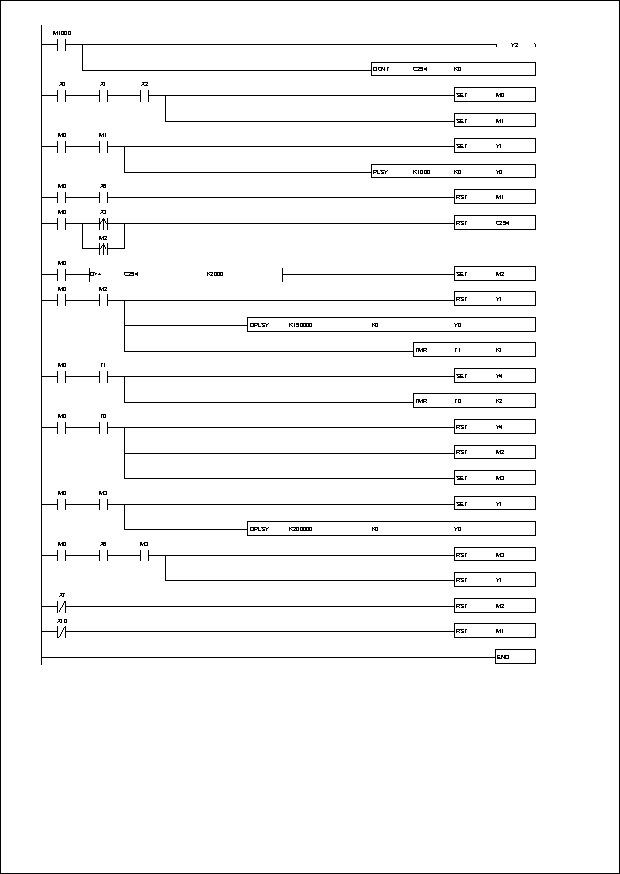
\includegraphics[width=\textwidth]{resources/code/flying_shear_code.pdf} 
    \caption[المخطط السلمي لخوارزمية المقص الطائر]{\centering المخطط السلمي لخوارزمية المقص الطائر، يوضح شبكات المزامنة، العدادات السريعة، وحماية نهايات الشوط.}
    \label{fig:ladder_code}
\end{figure}

\include{chapter/conclusion.tex}

%==================== المراجع ====================
\include{references/references}


\end{document}